%% AMS-LaTeX Created with the Wolfram Language : www.wolfram.com

\documentclass{article}
\usepackage{amsmath, amssymb, graphics, setspace}

\newcommand{\mathsym}[1]{{}}
\newcommand{\unicode}[1]{{}}

\newcounter{mathematicapage}
\begin{document}

\title{Tiling 3D Space}
\author{}
\date{}
\maketitle

I want to use the unit cell from the FCC lattice as the basis for 3D tiling for a rogue-like game movement in 3D. 

Lattice Vectors

The lattice vectors for the FCC lattice are typically written as:

\begin{doublespace}
\noindent\(\pmb{\text{a1}=\left\{\frac{1}{\sqrt{2}},\frac{1}{\sqrt{2}},0\right\};}\\
\pmb{\text{a2}=\left\{\frac{1}{\sqrt{2}},0,\frac{1}{\sqrt{2}}\right\};}\\
\pmb{\text{a3}=\left\{0,\frac{1}{\sqrt{2}},\frac{1}{\sqrt{2}}\right\};}\)
\end{doublespace}

This leads to the classic FCC packing for spheres.

\begin{doublespace}
\noindent\(\pmb{\text{Graphics3D}\left[\left\{\text{Blue},\text{Sphere}\left[\{0,0,0\},\frac{1}{2}\right],\right.\right.}\\
\pmb{\text{Red},\text{Translate}\left[\text{Sphere}\left[\{0,0,0\},\frac{1}{2}\right],\text{a1}\right],}\\
\pmb{\text{Green},\text{Translate}\left[\text{Sphere}\left[\{0,0,0\},\frac{1}{2}\right],\text{a2}\right],}\\
\pmb{\left.\text{Yellow},\text{Translate}\left[\text{Sphere}\left[\{0,0,0\},\frac{1}{2}\right],\text{a3}\right]\right\},\text{AxesOrigin}\to \{0,0,0\},\text{Axes}\to
\text{True},}\\
\pmb{\text{Boxed}\to \text{False}]}\)
\end{doublespace}

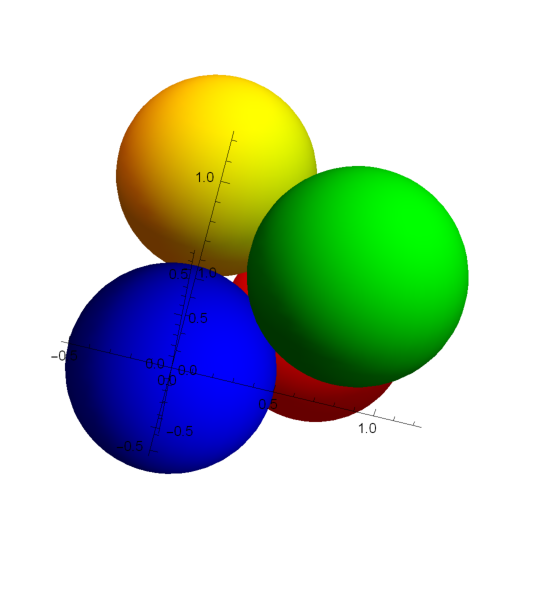
\includegraphics{3D_tiling_gr1.eps}

Rotated Lattic Vectors

I want to rotate these vectors so that one basis vector lies along the z axis and the other is in the xz plane. This will work well for the layout
I want to use in the game. \\
\\
The first step is to rotate the vectors so that one is along the z-axis. It turns out that rotating a2 is easy enough.

\begin{doublespace}
\noindent\(\pmb{\text{angle}=\text{ArcCos}[\text{Dot}[\text{a2},\{0,0,1\}]]}\\
\pmb{\text{rotVec}=\text{Cross}[\text{a2},\{0,0,1\}]}\\
\pmb{\text{rotMat} = \text{RotationMatrix}[\text{angle},\text{rotVec}] ;}\\
\pmb{\text{rotMat}\text{//}\text{MatrixForm}}\\
\pmb{\text{a1p} =\text{RotationMatrix}[0,\{0,0,1\}].\text{rotMat}.\text{a1}}\\
\pmb{\text{a2p} = \text{RotationMatrix}[0,\{0,0,1\}].\text{rotMat}.\text{a2}}\\
\pmb{\text{a3p} = \text{RotationMatrix}[0,\{0,0,1\}].\text{rotMat}.\text{a3}}\\
\pmb{\text{Graphics3D}[\{\text{Green},\text{Arrow}[\{\{0,0,0\},\text{a1p}\}],\text{Black},\text{Arrow}[\{\{0,0,0\},\text{a2p}\}],\text{Red},}\\
\pmb{\text{Arrow}[\{\{0,0,0\},\text{a3p}\}]\},\text{AxesOrigin}\to \{0,0,0\},\text{Axes}\to \text{True},\text{Boxed}\to \text{False},}\\
\pmb{\text{AxesLabel}\to \{x,y,z\},\text{ViewPoint}\to \{0,0,\infty \}]}\)
\end{doublespace}

\begin{doublespace}
\noindent\(\frac{\pi }{4}\)
\end{doublespace}

\begin{doublespace}
\noindent\(\left\{0,-\frac{1}{\sqrt{2}},0\right\}\)
\end{doublespace}

\begin{doublespace}
\noindent\(\left(
\begin{array}{ccc}
 \frac{1}{\sqrt{2}} & 0 & -\frac{1}{\sqrt{2}} \\
 0 & 1 & 0 \\
 \frac{1}{\sqrt{2}} & 0 & \frac{1}{\sqrt{2}} \\
\end{array}
\right)\)
\end{doublespace}

\begin{doublespace}
\noindent\(\left\{\frac{1}{2},\frac{1}{\sqrt{2}},\frac{1}{2}\right\}\)
\end{doublespace}

\begin{doublespace}
\noindent\(\{0,0,1\}\)
\end{doublespace}

\begin{doublespace}
\noindent\(\left\{-\frac{1}{2},\frac{1}{\sqrt{2}},\frac{1}{2}\right\}\)
\end{doublespace}

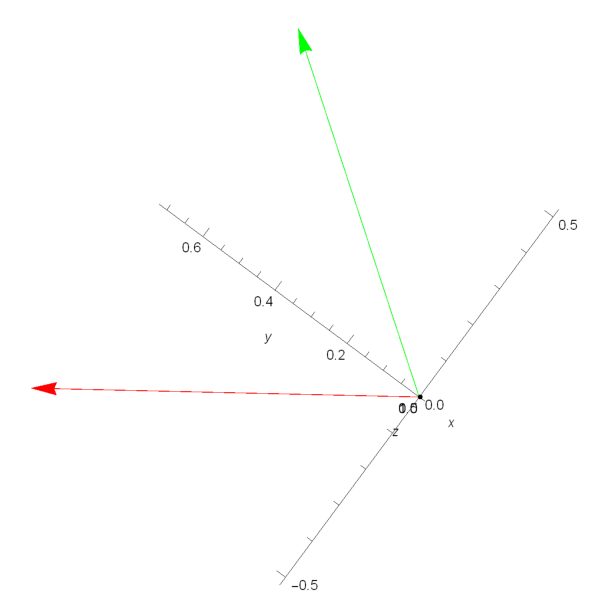
\includegraphics{3D_tiling_gr2.eps}

So, a \(\frac{-\pi }{4}\) rotation about the y-axis did the job.\\
Now I want one of the other two vectors to lie in the XZ plane (i.e. its Y coordinate is zero). To do this, I will project the green vector (a1p)
onto the xy plane, then use it to find the angle to rotate around the z-axis.

\begin{doublespace}
\noindent\(\pmb{\text{}}\\
\pmb{\text{a1proj}=\left\{\frac{1}{2},\frac{1}{\sqrt{2}},0\right\}/\text{Norm}\left[\left\{\frac{1}{2},\frac{1}{\sqrt{2}},0\right\}\right]}\)
\end{doublespace}

\begin{doublespace}
\noindent\(\left\{\frac{1}{\sqrt{3}},\sqrt{\frac{2}{3}},0\right\}\)
\end{doublespace}

\begin{doublespace}
\noindent\(\pmb{\text{angle2}=\text{ArcCos}[\text{Abs}[\text{Dot}[\text{a1proj},\{1,0,0\}]]]}\\
\pmb{\text{rotVec2}=\{0,0,-1\}}\\
\pmb{\text{rotMat2} = \text{RotationMatrix}[\text{angle2},\text{rotVec2}] ;}\\
\pmb{\text{rotMat2}\text{//}\text{MatrixForm}}\\
\pmb{\text{Print}[\text{{``}Basis Vector 1{''}}]}\\
\pmb{\text{a1p2} =\text{FullSimplify}[\text{rotMat2}.\text{a1p}]}\\
\pmb{\text{Print}[\text{{``}Basis Vector 2{''}}]}\\
\pmb{\text{a2p2} = \text{FullSimplify}[\text{rotMat2}.\text{a2p}]}\\
\pmb{\text{Print}[\text{{``}Basis Vector 3{''}}]}\\
\pmb{\text{a3p2} = \text{FullSimplify}[\text{rotMat2}.\text{a3p}]}\\
\pmb{\text{Graphics3D}[\{\text{Green},\text{Arrow}[\{\{0,0,0\},\text{a1p2}\}],\text{Black},\text{Arrow}[\{\{0,0,0\},\text{a2p2}\}],\text{Red},}\\
\pmb{\text{Arrow}[\{\{0,0,0\},\text{a3p2}\}]\},\text{AxesOrigin}\to \{0,0,0\},\text{Axes}\to \text{True},\text{Boxed}\to \text{False},}\\
\pmb{\text{AxesLabel}\to \{x,y,z\}]}\)
\end{doublespace}

\begin{doublespace}
\noindent\(\text{ArcCos}\left[\frac{1}{\sqrt{3}}\right]\)
\end{doublespace}

\begin{doublespace}
\noindent\(\{0,0,-1\}\)
\end{doublespace}

\begin{doublespace}
\noindent\(\left(
\begin{array}{ccc}
 \frac{1}{\sqrt{3}} & \sqrt{\frac{2}{3}} & 0 \\
 -\sqrt{\frac{2}{3}} & \frac{1}{\sqrt{3}} & 0 \\
 0 & 0 & 1 \\
\end{array}
\right)\)
\end{doublespace}

\noindent\(\text{Basis Vector 1}\)

\begin{doublespace}
\noindent\(\left\{\frac{\sqrt{3}}{2},0,\frac{1}{2}\right\}\)
\end{doublespace}

\noindent\(\text{Basis Vector 2}\)

\begin{doublespace}
\noindent\(\{0,0,1\}\)
\end{doublespace}

\noindent\(\text{Basis Vector 3}\)

\begin{doublespace}
\noindent\(\left\{\frac{1}{2 \sqrt{3}},\sqrt{\frac{2}{3}},\frac{1}{2}\right\}\)
\end{doublespace}

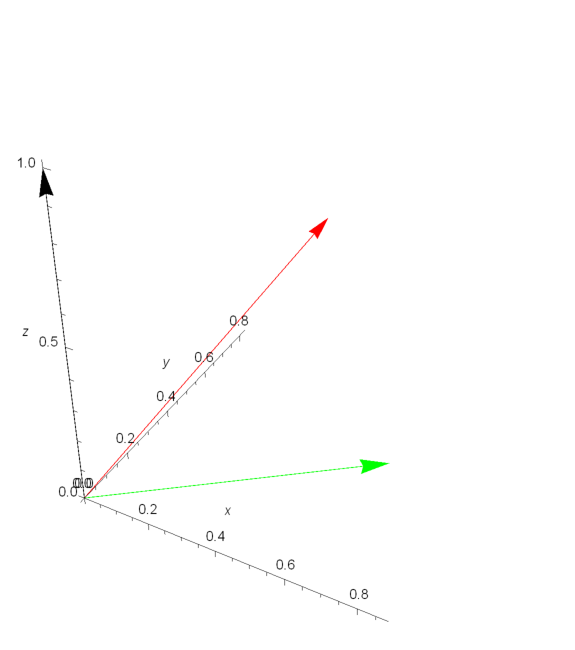
\includegraphics{3D_tiling_gr3.eps}

So it turns out that I needed to rotate it by the \(\text{ArcCos}\left[\sqrt{\frac{1}{3}}\right]\), which is an unusual angle, but it gives us what
we want. The total rotation matrix is:

\begin{doublespace}
\noindent\(\pmb{\text{rotMat2}.\text{rotMat}\text{//}\text{MatrixForm}}\)
\end{doublespace}

\begin{doublespace}
\noindent\(\left(
\begin{array}{ccc}
 \frac{1}{\sqrt{6}} & \sqrt{\frac{2}{3}} & -\frac{1}{\sqrt{6}} \\
 -\frac{1}{\sqrt{3}} & \frac{1}{\sqrt{3}} & \frac{1}{\sqrt{3}} \\
 \frac{1}{\sqrt{2}} & 0 & \frac{1}{\sqrt{2}} \\
\end{array}
\right)\)
\end{doublespace}

Just to have them, I{'}m converting the basis vectors into decimal form.

\begin{doublespace}
\noindent\(\pmb{N[\{\text{a1p2},\text{a2p2},\text{a3p2}\}]}\)
\end{doublespace}

\begin{doublespace}
\noindent\(\{\{0.866025,0.,0.5\},\{0.,0.,1.\},\{0.288675,0.816497,0.5\}\}\)
\end{doublespace}

And we check the unit lattice.

\begin{doublespace}
\noindent\(\pmb{\text{Graphics3D}[}\\
\pmb{\text{Flatten}\left[\left\{\text{Opacity}[0.3],\text{Table}\left[\text{Translate}\left[\text{Sphere}\left[\{0,0,0\},\frac{1}{2}\right],\{u \text{a1p}
+ v \text{a2p} + w \text{a3p}\}\right],\right.\right.\right.}\\
\pmb{\{u,-2,2\},\{v,0,2\},\{w,-2,2\}]\}],\text{AxesOrigin}\to \{0,0,0\},\text{Axes}\to \text{True},\text{Boxed}\to \text{False}]}\)
\end{doublespace}

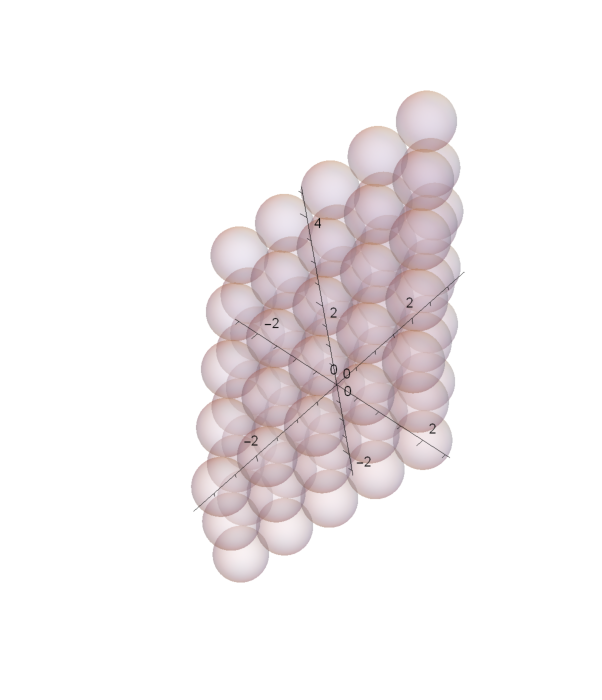
\includegraphics{3D_tiling_gr4.eps}

Tiling Polyhedra

I now want to tile space with the rhombic dodecahedron. The FCC Vornois tesellation is the Rhomic dodcahedron, so this should mesh perfectly with
our new basis vectors.\\
\\
We first visualize this shape.

\begin{doublespace}
\noindent\(\pmb{\text{PolyhedronData}[\text{{``}RhombicDodecahedron{''}}]}\)
\end{doublespace}

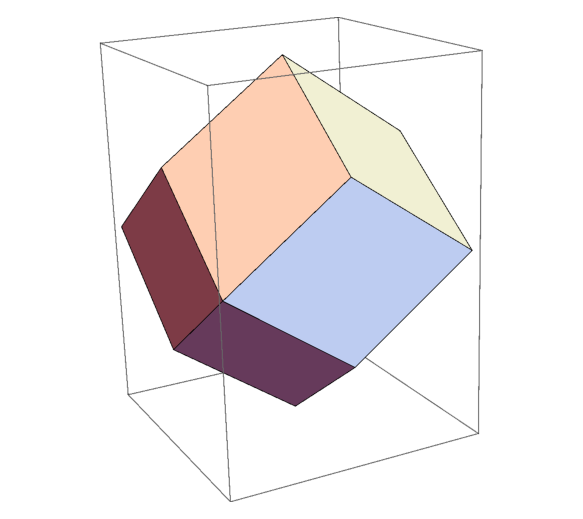
\includegraphics{3D_tiling_gr5.eps}

We check the tesellation of this shape using our basis vectors.

\begin{doublespace}
\noindent\(\pmb{\text{Graphics3D}[\{\text{Blue},\text{PolyhedronData}[\text{{``}RhombicDodecahedron{''}},\text{{``}Faces{''}}],}\\
\pmb{\text{Red},\text{Translate}[\text{PolyhedronData}[\text{{``}RhombicDodecahedron{''}},\text{{``}Faces{''}}],\text{a1p2}],}\\
\pmb{\text{Green},\text{Translate}[\text{PolyhedronData}[\text{{``}RhombicDodecahedron{''}},\text{{``}Faces{''}}],\text{a2p2}],}\\
\pmb{\text{Yellow},\text{Translate}[\text{PolyhedronData}[\text{{``}RhombicDodecahedron{''}},\text{{``}Faces{''}}],\text{a3p2}]\},}\\
\pmb{\text{AxesOrigin}\to \{0,0,0\},\text{Axes}\to \text{True},\text{Boxed}\to \text{False}]}\)
\end{doublespace}

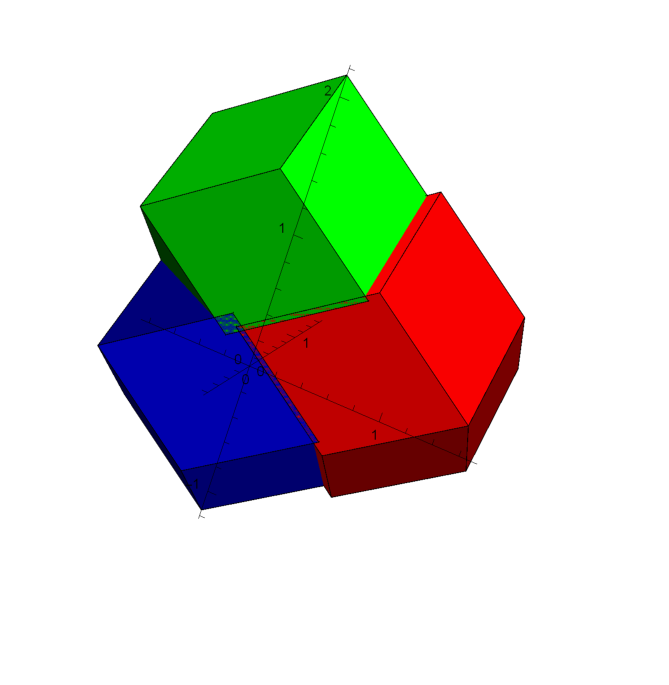
\includegraphics{3D_tiling_gr6.eps}

First step, it looks like the dodecahera are too large for a unit translation. Let{'}s get the scale.

\begin{doublespace}
\noindent\(\pmb{\text{PolyhedronData}[\text{{``}RhombicDodecahedron{''}},\text{{``}Insphere{''}}]}\)
\end{doublespace}

\begin{doublespace}
\noindent\(\text{Sphere}\left[\{0,0,0\},\sqrt{\frac{2}{3}}\right]\)
\end{doublespace}

As suspected, the radius of the inscribe sphere is not \(\frac{1}{2}\) (unit diameter). Fixing that:

\begin{doublespace}
\noindent\(\pmb{\text{Graphics3D}\left[\left\{\text{Scale}\left[\text{PolyhedronData}[\text{{``}RhombicDodecahedron{''}},\text{{``}Insphere{''}}],\frac{1}{2}\sqrt{\frac{3}{2}}\right],\right.\right.}\\
\pmb{\left.\text{Scale}\left[\text{PolyhedronData}[\text{{``}RhombicDodecahedron{''}},\text{{``}Edges{''}}],\frac{1}{2}\sqrt{\frac{3}{2}}\right]\right\},\text{AxesOrigin}\to
\{0,0,0\},}\\
\pmb{\text{Axes}\to \text{True},\text{Boxed}\to \text{False}]}\)
\end{doublespace}

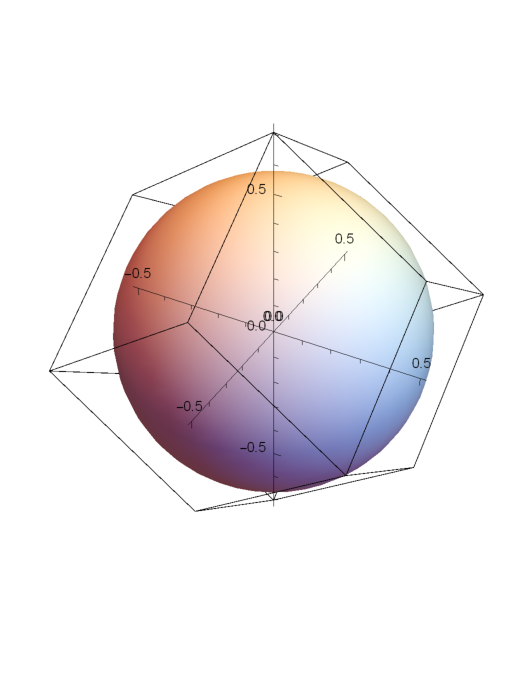
\includegraphics{3D_tiling_gr7.eps}

That looks better. Let{'}s try the tesellation again with the re-sized polyhedra.

\begin{doublespace}
\noindent\(\pmb{\text{Graphics3D}\left[\left\{\text{Blue},\text{Scale}\left[\text{PolyhedronData}[\text{{``}RhombicDodecahedron{''}},\text{{``}Faces{''}}],\frac{1}{2}\sqrt{\frac{3}{2}}\right],\right.\right.}\\
\pmb{\text{Red},\text{Translate}\left[\text{Scale}\left[\text{PolyhedronData}[\text{{``}RhombicDodecahedron{''}},\text{{``}Faces{''}}],\frac{1}{2}\sqrt{\frac{3}{2}}\right],\text{a1p2}\right],}\\
\pmb{\text{Green},\text{Translate}\left[\text{Scale}\left[\text{PolyhedronData}[\text{{``}RhombicDodecahedron{''}},\text{{``}Faces{''}}],\frac{1}{2}\sqrt{\frac{3}{2}}\right],\text{a2p2}\right],}\\
\pmb{\left.\text{Yellow},\text{Translate}\left[\text{Scale}\left[\text{PolyhedronData}[\text{{``}RhombicDodecahedron{''}},\text{{``}Faces{''}}],\frac{1}{2}\sqrt{\frac{3}{2}}\right],\text{a3p2}\right]\right\},}\\
\pmb{\text{AxesOrigin}\to \{0,0,0\},\text{Axes}\to \text{True},\text{Boxed}\to \text{False},\text{AxesLabel}\to \{x,y,z\}]}\)
\end{doublespace}

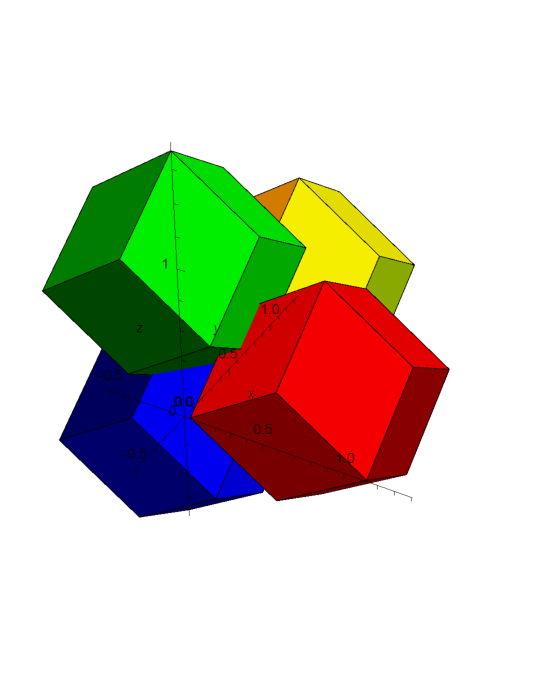
\includegraphics{3D_tiling_gr8.eps}

That fixed the scale problem. Now the rotation of the dodecahedron is off. I want the tiling to match faces. This requres two rotations. First, we
rotate by \(\frac{\pi }{2}\) around the y-axis. Then we have to do a second rotation that turns out to be a rotation of \(\text{ArcCos}\left[\sqrt{\frac{2}{3}}\right]\)
radians around the z-axis. We then look at the projections in all three directions to make sure that things are tiled correctly.

\begin{doublespace}
\noindent\(\pmb{\text{rotationAngle} = \frac{\pi }{2};}\\
\pmb{\text{rotationVector}=\{0,1,0\};}\\
\pmb{\text{MakePoly}[\text{transVec$\_$}]\text{:=}}\\
\pmb{\text{Translate}[\text{GeometricTransformation}[}\\
\pmb{\text{GeometricTransformation}\left[\text{Scale}\left[\text{PolyhedronData}[\text{{``}RhombicDodecahedron{''}},\text{{``}Edges{''}}],\frac{1}{2}\sqrt{\frac{3}{2}}\right],\right.}\\
\pmb{\left.\text{RotationMatrix}[\text{rotationAngle},\text{rotationVector}]],\text{RotationMatrix}\left[\text{ArcCos}\left[\sqrt{\frac{2}{3}}\right],\{0,0,1\}\right]\right],}\\
\pmb{\text{transVec}];}\\
\pmb{}\\
\pmb{\text{GraphicsGrid}[\{\{\text{Graphics3D}[\{\text{Blue},\text{MakePoly}[\{0,0,0\}],}\\
\pmb{\text{Red},\text{MakePoly}[\text{a1p2}],}\\
\pmb{\text{Green},\text{MakePoly}[\text{a2p2}],}\\
\pmb{\text{Yellow},\text{MakePoly}[\text{a3p2}]\},\text{AxesOrigin}\to \{0,0,0\},\text{Axes}\to \text{True},\text{Boxed}\to \text{False},}\\
\pmb{\text{AxesLabel}\to \{x,y,z\},\text{ViewPoint}\to \{\infty ,0,0\}],}\\
\pmb{\text{Graphics3D}[\{\text{Blue},\text{MakePoly}[\{0,0,0\}],}\\
\pmb{\text{Red},\text{MakePoly}[\text{a1p2}],}\\
\pmb{\text{Green},\text{MakePoly}[\text{a2p2}],}\\
\pmb{\text{Yellow},\text{MakePoly}[\text{a3p2}]\},\text{AxesOrigin}\to \{0,0,0\},\text{Axes}\to \text{True},\text{Boxed}\to \text{False},}\\
\pmb{\text{AxesLabel}\to \{x,y,z\},\text{ViewPoint}\to \{0,\infty ,0\}],}\\
\pmb{\text{Graphics3D}[\{\text{Blue},\text{MakePoly}[\{0,0,0\}],}\\
\pmb{\text{Red},\text{MakePoly}[\text{a1p2}],}\\
\pmb{\text{Green},\text{MakePoly}[\text{a2p2}],}\\
\pmb{\text{Yellow},\text{MakePoly}[\text{a3p2}]\},\text{AxesOrigin}\to \{0,0,0\},\text{Axes}\to \text{True},\text{Boxed}\to \text{False},}\\
\pmb{\text{AxesLabel}\to \{x,y,z\},\text{ViewPoint}\to \{0,0,\infty \}]\}\},\text{ImageSize}\to \text{Large}]}\)
\end{doublespace}

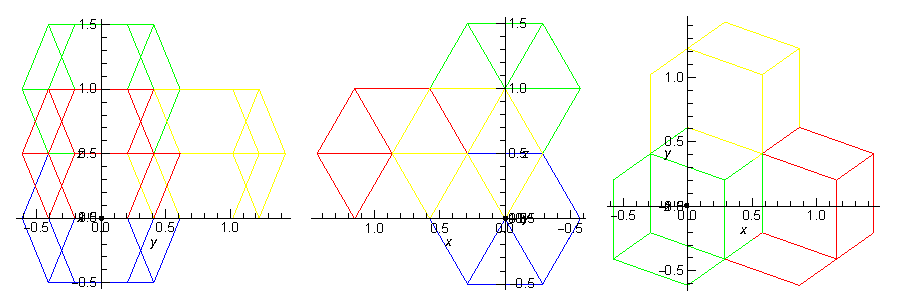
\includegraphics{3D_tiling_gr9.eps}

And we check the tiling in 3D to make sure it looks good.

\begin{doublespace}
\noindent\(\pmb{\text{MakePolyFace}[\text{transVec$\_$}]\text{:=}}\\
\pmb{\text{Translate}[\text{GeometricTransformation}[}\\
\pmb{\text{GeometricTransformation}\left[\text{Scale}\left[\text{PolyhedronData}[\text{{``}RhombicDodecahedron{''}},\text{{``}Faces{''}}],\frac{1}{2}\sqrt{\frac{3}{2}}\right],\right.}\\
\pmb{\left.\text{RotationMatrix}[\text{rotationAngle},\text{rotationVector}]],\text{RotationMatrix}\left[\text{ArcCos}\left[\sqrt{\frac{2}{3}}\right],\{0,0,1\}\right]\right],}\\
\pmb{\text{transVec}];}\\
\pmb{\text{Graphics3D}[\{\text{Blue},\text{MakePolyFace}[\{0,0,0\}],}\\
\pmb{\text{Red},\text{MakePolyFace}[\text{a1p2}],}\\
\pmb{\text{Green},\text{MakePolyFace}[\text{a2p2}],}\\
\pmb{\text{Yellow},\text{MakePolyFace}[\text{a3p2}]\},\text{AxesOrigin}\to \{0,0,0\},\text{Axes}\to \text{True},\text{Boxed}\to \text{False},}\\
\pmb{\text{AxesLabel}\to \{x,y,z\}]}\)
\end{doublespace}

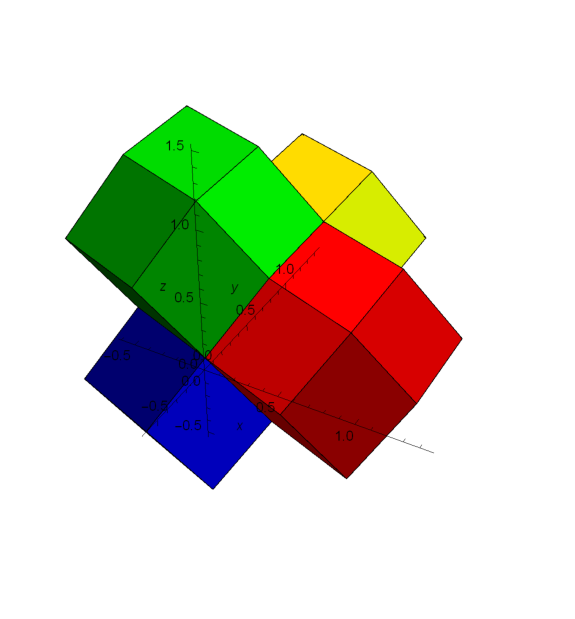
\includegraphics{3D_tiling_gr10.eps}

These two rotations now give us the coordinates for all of the vertices for the rhombic dodecahedron in our basis.

\begin{doublespace}
\noindent\(\pmb{\text{points}=}\\
\pmb{\text{FullSimplify}\left[\text{Map}\left[ \frac{1}{2}\sqrt{\frac{3}{2}}\text{RotationMatrix}\left[\text{ArcCos}\left[\sqrt{\frac{2}{3}}\right],\{0,0,1\}\right].\text{RotationMatrix}\left[\frac{\pi
}{2},\{0,1,0\}\right].\#\&,\right.\right.}\\
\pmb{\text{PolyhedronData}[\text{{``}RhombicDodecahedron{''}},\text{{``}VertexCoordinates{''}}]]];}\\
\pmb{\text{Transpose}@\{\text{PolyhedronData}[\text{{``}RhombicDodecahedron{''}},\text{{``}VertexIndices{''}}], \text{points}\}\text{//}\text{MatrixForm}}\)
\end{doublespace}

\begin{doublespace}
\noindent\(\left(
\begin{array}{cc}
 1 & \left\{\frac{1}{2 \sqrt{3}},-\frac{1}{\sqrt{6}},\frac{1}{2}\right\} \\
 2 & \left\{-\frac{1}{2 \sqrt{3}},-\frac{1}{2 \sqrt{6}},\frac{1}{2}\right\} \\
 3 & \left\{\frac{1}{2 \sqrt{3}},\frac{1}{2 \sqrt{6}},\frac{1}{2}\right\} \\
 4 & \left\{-\frac{1}{2 \sqrt{3}},\frac{1}{\sqrt{6}},\frac{1}{2}\right\} \\
 5 & \left\{0,-\frac{\sqrt{\frac{3}{2}}}{2},0\right\} \\
 6 & \left\{\frac{1}{\sqrt{3}},-\frac{1}{2 \sqrt{6}},0\right\} \\
 7 & \left\{-\frac{1}{\sqrt{3}},-\frac{1}{\sqrt{6}},0\right\} \\
 8 & \left\{\frac{1}{\sqrt{3}},\frac{1}{\sqrt{6}},0\right\} \\
 9 & \left\{-\frac{1}{\sqrt{3}},\frac{1}{2 \sqrt{6}},0\right\} \\
 10 & \left\{0,\frac{\sqrt{\frac{3}{2}}}{2},0\right\} \\
 11 & \left\{\frac{1}{2 \sqrt{3}},-\frac{1}{\sqrt{6}},-\frac{1}{2}\right\} \\
 12 & \left\{-\frac{1}{2 \sqrt{3}},-\frac{1}{2 \sqrt{6}},-\frac{1}{2}\right\} \\
 13 & \left\{\frac{1}{2 \sqrt{3}},\frac{1}{2 \sqrt{6}},-\frac{1}{2}\right\} \\
 14 & \left\{-\frac{1}{2 \sqrt{3}},\frac{1}{\sqrt{6}},-\frac{1}{2}\right\} \\
\end{array}
\right)\)
\end{doublespace}

\begin{doublespace}
\noindent\(\pmb{\text{Show}[}\\
\pmb{\text{Graphics3D}[\text{GeometricTransformation}[}\\
\pmb{\text{GeometricTransformation}\left[\text{Scale}\left[\text{PolyhedronData}[\text{{``}RhombicDodecahedron{''}},\text{{``}Edges{''}}],\frac{1}{2}\sqrt{\frac{3}{2}}\right],\right.}\\
\pmb{\left.\text{RotationMatrix}[\text{rotationAngle},\text{rotationVector}]],\text{RotationMatrix}\left[\text{ArcCos}\left[\sqrt{\frac{2}{3}}\right],\{0,0,1\}\right]\right],}\\
\pmb{\text{Boxed}\to \text{False}],}\\
\pmb{\text{Graphics3D}[}\\
\pmb{\{\text{MapThread}[\text{Text}[\text{Style}[\text{$\#$1},\text{Bold},\text{Large},\text{Red}],\text{$\#$2}]\&,}\\
\pmb{\{\text{PolyhedronData}[\text{{``}RhombicDodecahedron{''}},\text{{``}VertexIndices{''}}],\text{points}\}]\}]]}\)
\end{doublespace}

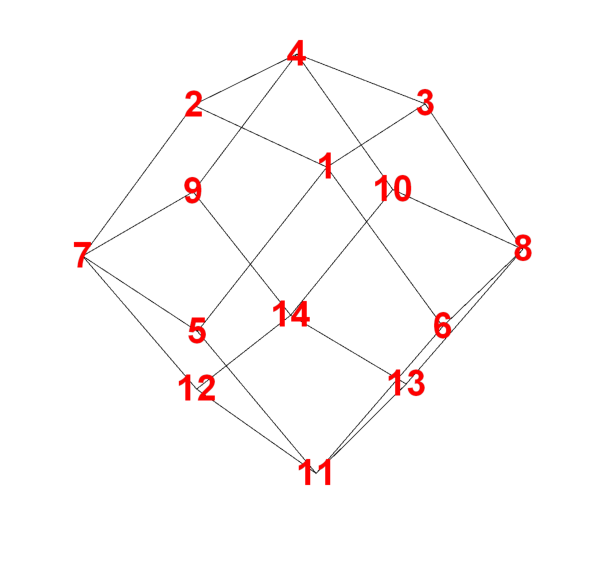
\includegraphics{3D_tiling_gr11.eps}

Finally, we get the numerical values of the points for translation to the video game.

\begin{doublespace}
\noindent\(\pmb{\text{Transpose}@\{\text{PolyhedronData}[\text{{``}RhombicDodecahedron{''}},\text{{``}VertexIndices{''}}], N[\text{points}]\}\text{//}}\\
\pmb{\text{MatrixForm}}\)
\end{doublespace}

\begin{doublespace}
\noindent\(\left(
\begin{array}{cc}
 1 & \{0.288675,-0.408248,0.5\} \\
 2 & \{-0.288675,-0.204124,0.5\} \\
 3 & \{0.288675,0.204124,0.5\} \\
 4 & \{-0.288675,0.408248,0.5\} \\
 5 & \{0.,-0.612372,0.\} \\
 6 & \{0.57735,-0.204124,0.\} \\
 7 & \{-0.57735,-0.408248,0.\} \\
 8 & \{0.57735,0.408248,0.\} \\
 9 & \{-0.57735,0.204124,0.\} \\
 10 & \{0.,0.612372,0.\} \\
 11 & \{0.288675,-0.408248,-0.5\} \\
 12 & \{-0.288675,-0.204124,-0.5\} \\
 13 & \{0.288675,0.204124,-0.5\} \\
 14 & \{-0.288675,0.408248,-0.5\} \\
\end{array}
\right)\)
\end{doublespace}

\end{document}
